\label{sec:evaluation}
% TODO: Explain why we don't evaluate on parallel programs

We evaluate \doubletake{} to demonstrate its efficiency, both in runtime and memory overhead. We also demonstrate the effectiveness of our detection tools across a benchmark suite and with several real applications. All experiments are run on a quiescent Intel Core 2 dual-processor system with 16GB of RAM running Linux 2.6.18, and version 2.5 of \texttt{glibc}. Each processor is a 4-core 64-bit Intel Xeon, operating at 2.33GHz with a 4MB shared L2 cache a 32KB per-core L1 cache. All benchmarks are built as 64-bit executables using LLVM 3.2 with the clang front-end and \texttt{-O2} optimizations.

% -194.17.1.el5

Our evaluation measures the memory and runtime overhead of \doubletake{}, and the effectiveness of the heap buffer overflow, memory leak, and use-after-free detectors.

\subsection{Runtime Overhead}
\label{sec:evaluation/runtime}

\begin{table}[!t]
	\centering
	\begin{tabular}{l|r p{0.1em} l|r}
		\textbf{Benchmark} & \textbf{Overhead} & & \textbf{Benchmark} & \textbf{Overhead} \\
		\cline{1-2} \cline{4-5}
		400.perlbench	& 20.5$\times$	& & 458.sjeng	& 20.3$\times$	\\
		401.bzip2		& 16.8$\times$	& & 471.omnetpp	& 13.9$\times$	\\
		403.gcc			& 18.7$\times$	& & 473.astar	& 11.9$\times$	\\
		429.mcf			& 4.5$\times$ 	& & 433.milc		& 11.0$\times$	\\
		445.gobmk		& 28.9$\times$	& & 444.namd		& 24.9$\times$	\\
		456.hmmer		& 13.8$\times$	& & 450.dealII	& 42.8$\times$	\\
	\end{tabular}
	\caption{Valgrind runtime overhead. \label{table:valgrind}}
\end{table}


\begin{table}[!t]
\centering
\begin{tabular}{l|r| r| r|r }
\textbf{Benchmark} & \textbf{Processes} & \textbf{Epochs} & \textbf{Syscalls} & \textbf{Mallocs (\#)} \\
\hline
400.perlbench & 3 & 291 & 60068 & 360605640 \\
401.bzip2 & 6 & 6 & 968 & 168 \\
403.gcc & 9 & 9 & 155505 & 28458514 \\
429.mcf & 1 & 1 & 24443 & 5 \\
445.gobmk & 5 & 5 & 2248 & 658034 \\
456.hmmer & 2 & 2 & 46 & 2474268 \\
458.sjeng & 1 & 1 & 23 & 5 \\
462.libquantum & 1 & 1 & 11 & 179 \\
464.h264ref & 3 & 885 & 2592 & 146827 \\
471.omnetpp & 1 & 1 & 19 & 267168472 \\
473.astar & 2 & 2 & 102 & 4799955 \\
483.xalancbmk & 1 & 1 & 123706 & 135155557 \\
433.milc & 1 & 1 & 12 & 6517 \\
444.namd & 1 & 1 & 470 & 1324 \\
447.dealII & 1 & 1 & 8131 & 151332314 \\
450.soplex & 2 & 2 & 37900 & 310619 \\
453.povray & 1 & 1 & 25721 & 2461141 \\	
\end{tabular}
\caption{Benchmark characteristics. \label{table:character}}
\end{table}


The runtime and memory overhead of \doubletake{} is evaluated with all C and C++ SPEC CPU2006 benchmarks, 19 in total. We compare \doubletake{} with AddressSanitizer and Valgrind. AddressSanitizer is the previous state-of-the-art for detecting buffer overflows and use-after-free errors, but cannot detect memory leaks~\cite{AddressSanitizer}. Valgrind's Memcheck tool is widely used to detect buffer overflows, memory leaks, and use-after-free errors~\cite{overflow:valgrind}. 

\begin{figure*}[ht!]
\begin{center}
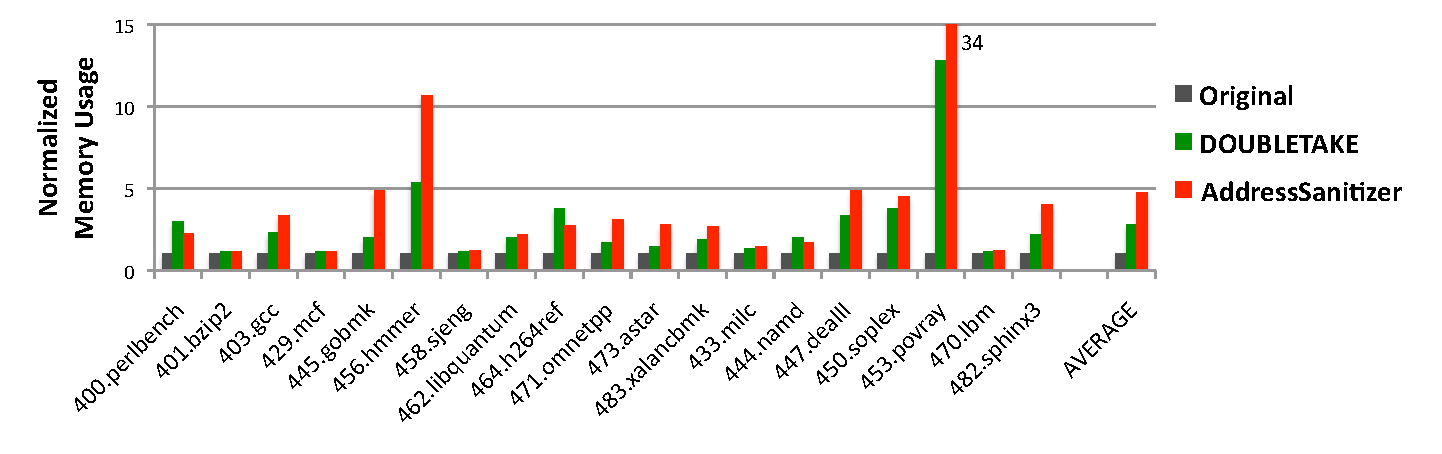
\includegraphics[width=6.5in]{figure/memory}
\end{center}
\caption{
Memory overhead of \doubletake{} and AddressSanitizer.
\label{fig:memory}}
\end{figure*}

During performance evaluation, we disable \doubletake{}'s rollback to measure only the overhead of normal execution. \doubletake{}'s memory error detectors only run on the heap, so AddressSanitizer is configured to check only writes to heap memory. For each benchmark, we report the average of three runs with the largest input size, except for Valgrind. We only run Valgrind once because of its high runtime overhead. 

Figure~\ref{fig:perf} shows the runtime overhead results for \doubletake{} and AddressSanitizer. Results for Valgrind do not fit on the graph, and are presented separately in Table~\ref{table:valgrind}. On average, \doubletake{} adds only $9\%$ overhead \emph{with all three error detectors enabled}. Without use-after-free detection, \doubletake{}'s overhead is just $3\%$. Overflow detection alone slows execution by just $2\%$. AddressSanitizer has an average runtime overhead of $30\%$. Valgrind has an average runtime overhead of $20\times$, but two benchmarks (\texttt{perlbench} and \texttt{sjeng}) have not yet finished running.

% difference across all different tools
For 17 out of 19 benchmarks, \doubletake{} outperforms AddressSanitizer, even with memory leak detection enabled. For 12 benchmarks, \doubletake{}'s runtime overhead with all detectors enabled is under 3\%. Both \doubletake{} and AddressSanitizer substantially outperform Valgrind on all benchmarks. Three benchmarks, \texttt{400.perlbench}, \texttt{403.gcc} and \texttt{447.dealII}, have substantially higher overhead than most benchmarks with both \doubletake{} and AddressSanitizer. Table~\ref{tbl:memoryoverhead} shows that \doubletake{} and AddressSanitizer both add substantial memory overhead for these benchmarks. This increased memory footprint is likely responsible for the degraded performance due to increased cache and TLB pressure.

% Difference across all different tools
\doubletake{}'s use-after-free detection adds roughly $6\%$ runtime overhead: only \texttt{perlbench}, \texttt{gcc}, and \texttt{h264ref} run with more than $20\%$ overhead. As described in Section~\ref{sec:applications/useafterfree}, all freed objects are filled with canaries (up to 128 bytes). \doubletake{} spends a substantial amount of time filling freed memory with canaries for applications with a large number of \texttt{malloc} and \texttt{free} calls.

Table~\ref{table:character} shows detailed benchmark characteristics. The ``Processes'' column shows the number of different invocations in the input set. The number of epochs is significantly lower than the number of system calls because of \doubletake{}'s lightweight system call handling. Benchmarks with the highest overhead run a substantial number of epochs (\texttt{perlbench} and \texttt{h264ref}) and make a large number of \texttt{malloc} calls (\texttt{gcc}, \texttt{omnetpp}, and \texttt{xalancbmk}).

%%%%%%%%%%%%%%%%%%%%%%%%%%%%%%%

\subsection{Memory Overhead}
\label{sec:evaluation/memory}

Much of \doubletake{}'s memory overhead comes from the snapshot of writable memory at the beginning at each epoch. However, the first snapshot is very small because the heap is completely empty. The benchmarks \texttt{bzip2}, \texttt{mcf}, \texttt{sjeng}, \texttt{milc}, and \texttt{lbm} run in a single epoch, and therefore have very low memory overhead. System call logs introduce a small amount of additional overhead. Other sources of memory overhead are application-specific: buffer overflow detection adds space between heap objects, which can increase memory usage for programs with many small allocations. Use-after-free detection adds constant-size memory overhead by delaying memory reuse.

Figure~\ref{fig:memory} shows memory overhead for \doubletake{} and AddressSanitizer, and Table~\ref{tbl:memoryoverhead} contains a detailed breakdown. We measure program memory usage by recording the peak \emph{physical} memory usage because \doubletake{}'s pre-allocated heap consumes 4GB of virtual memory. Peak memory usage is collected by periodically sampling the proportional set size files (\texttt{/proc/self/smaps}).

On average, \doubletake{} imposes $2.8\times$ memory overhead, while AddressSanitizer introduces $4.8\times$ overhead. For \texttt{povray} and \texttt{h264ref}, both tools introduce large relative memory overhead because these benchmarks use just 3MB and 24MB respectively. Complete memory usage results are shown in Table~\ref{tbl:memoryoverhead}. For all other benchmarks, both \doubletake{} and AddressSanitizer introduce less than $5\times$ memory overhead. \doubletake{} has lower memory overhead than AddressSanitizer on all but two benchmarks: \texttt{perlbench} and \texttt{namd}. \doubletake{}'s total memory usage is less than twice that of the original programs, and $20\%$ less than AddressSanitizer. 

\begin{table}[h!]
\centering
\begin{tabular}{l|r|r|r}
\textbf{ \small Benchmark} & \textbf{\small Original} &  \textbf{\small AddressSanitizer} & \textbf{\small \doubletake{} } \\
\hline
400.perlbench & 656 &	1481 & 1977 \\
401.bzip2	& 870 &	1020 &	1003 \\
403.gcc	& 683 &	2293 &	1583 \\
429.mcf	& 1716 &	1951 &	1994 \\
445.gobmk &	28 &	137 &	58 \\
456.hmmer &	24 &	256 &	129 \\
458.sjeng & 179 & 220 &	203 \\
462.libquantum	& 66 &	144 &	131 \\
464.h264ref	& 65 &	179 &	247 \\
471.omnetpp	& 172 &	538 &	291 \\
473.astar	& 333 &	923 &	477 \\
483.xalancbmk &	428 & 1149 &	801 \\
433.milc	& 695 &	1008 &	917 \\
444.namd	& 46 &	79 &	92 \\
447.dealII	& 514 &	2496 &	1727 \\
450.soplex	& 441 &	1991 &	1654 \\
453.povray	& 3 &	133 &	50 \\
470.lbm	& 418 &	496 &	470 \\
482.sphinx3 &	45 &	181 & 98 \\
\hline
\textbf{Total} & \textbf{7386} & \textbf{16678} & \textbf{13906} \\
\end{tabular}
\caption{\doubletake{} and AddressSanitizer memory use (MB).\label{tbl:memoryoverhead}}
\end{table}


%%%%%%%%%%%%%%%%%%%%%%%%%%%%%%%

\subsection{Effectiveness}
\label{sec:effect}

We use \doubletake{} to find errors in both the SPEC CPU2006 benchmark suite and a suite of real applications.

\paragraph{Benchmarks.}
\doubletake{} detected a one-byte heap buffer overflow in \texttt{perlbench}, which is not detected by AddressSanitizer. \doubletake{} also detected a significant number of memory leaks in \texttt{perlbench} and \texttt{gcc}, which we have verified using Valgrind's Memcheck tool.

\paragraph{Real applications.}
\doubletake{} detects known buffer overflows in \texttt{libHX}, \texttt{bzip2}, \texttt{vim},\texttt{bc}, \texttt{polymorph}, and \texttt{gzip}. Buggy inputs were obtained from prior buffer overflow detection tools, Red Hat's Bugzilla, and bugbench~\cite{vimoverflow, bzip2overflow,bugbench,overflow:Cruiser}.

The buffer overflows we observed in these applications are triggered by specific inputs, which are difficult to detect during development. In most cases, \doubletake{}'s overhead is low enough to be enabled in deployment, which would make it possible to detect these bugs in the field.  \doubletake{} also detects memory leaks in \texttt{gcc-4.4.7} and \texttt{vim}.
